\section{Theory}
\subsection{The Transmission electron microscope}
The Transmission electron microscope (TEM) is a microscope that far exceeds the capabilities of a normal light microscope. Both types of microscope use a series of lenses to magnify the image of a specimen.
A normal light microscope can amplify an image up to about 1500$\times$ and is limited by the diffraction limit. Assuming an average wavelength of 550$nm$ for green light a high-end microscope is limited to resolving features 100$nm$ apart.
This limit is too low for looking at atomic structures.\cite{PhysRevLett.106.193905}\\
An electron microscope circumvents this limit by using electrons, not light, to probe the specimen. Electrons when accelerated have a smaller wavelength than light thus allowing for images with resolved features as small as 0.05$nm$. \cite{kisielowski_freitag_bischoff_van}
The TEM works by releasing electrons from an electron source and accelerating them to an energy typically expressed in kilo-electronvolt. After being accelerated the electrons pass multiple electromagnetic lenses and a condenser aperture to shape the beam before it 'illuminates' the specimen as illustrated in \ref{fig:tem}.
The beam incident on the sample is limited to a illumination semi-angle $\alpha$ which is inversely proportional to the resolution, but limiting $\alpha$ decreases the amount of electrons incident on the specimen and thus a frame needs more time for a decent exposure.
After having interacted with the specimen the beam is again limited by an aperture, this aperture sets the collection semi-angle $\beta$ which controls the limit of scattering angles allowed into the imaging lenses.
After the beam is conditioned by the imaging lenses it passes trough four electromagnetic prisms which make up an energy filter called an $\Omega$-filter named after the shape it needs to have to keep the TEM stack aligned with the CCD-camera to limit aberrations.
The $\Omega$-filter is used for energy filtered TEM images discussed in \ref{sec:eftem}.\\
Two types of images can be made with the TEM, a normal image which shows the magnified sample and a diffraction pattern image which can be made by placing the capture device in the focal point of the lens and filter system.
A diffraction mode image shows the diffraction peaks that are characteristic of the sample and yields information on the reciprocal lattice of the sample.


%+ Normal microscope
%+ Electron microscope resolution
%+ Workings with diagram
%+ Imaging modes


\begin{figure}
	\centering
	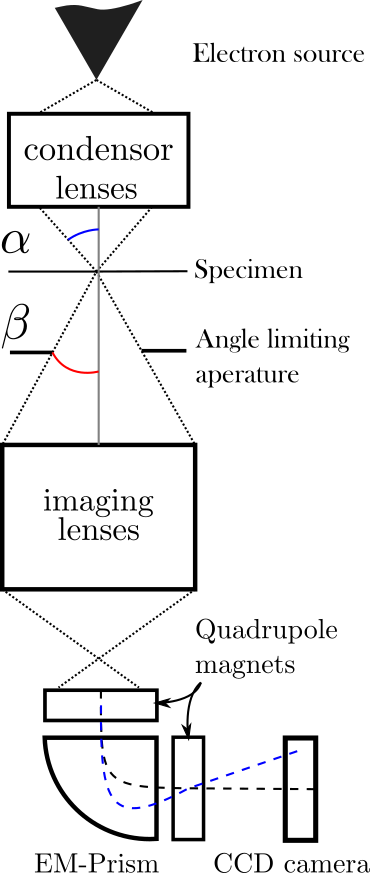
\includegraphics[width=0.25\linewidth, keepaspectratio]{tem.png}
	\caption{TEM}
	\label{fig:tem}
\end{figure}

\subsection{Electron scattering theory}


\begin{figure}
	\centering
	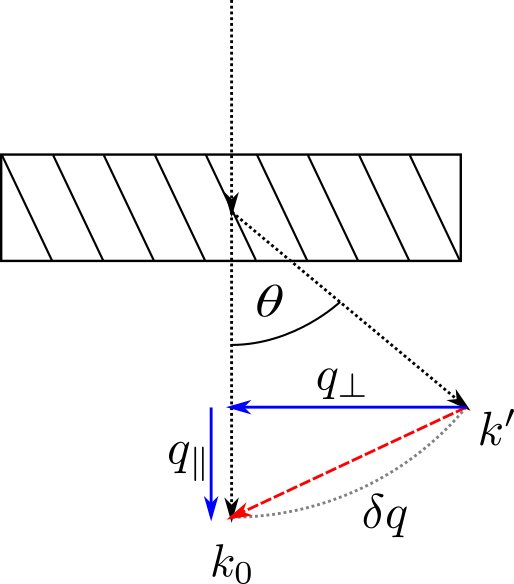
\includegraphics[width=0.25\linewidth, keepaspectratio]{scat.png}
	\caption{scat}
	\label{fig:scat}
\end{figure}


\subsection{Momentum resolved electron energy-loss spectroscopy}

\begin{figure}
	\centering
	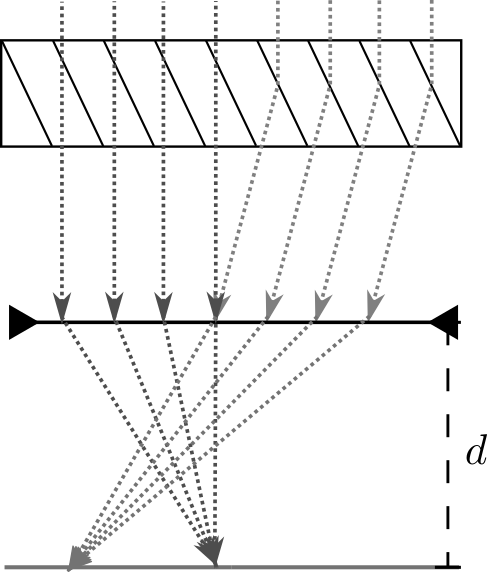
\includegraphics[width=0.25\linewidth, keepaspectratio]{diff-im.png}
	\caption{scat}
	\label{fig:diff-im}
\end{figure}
\begin{figure}
	\centering
	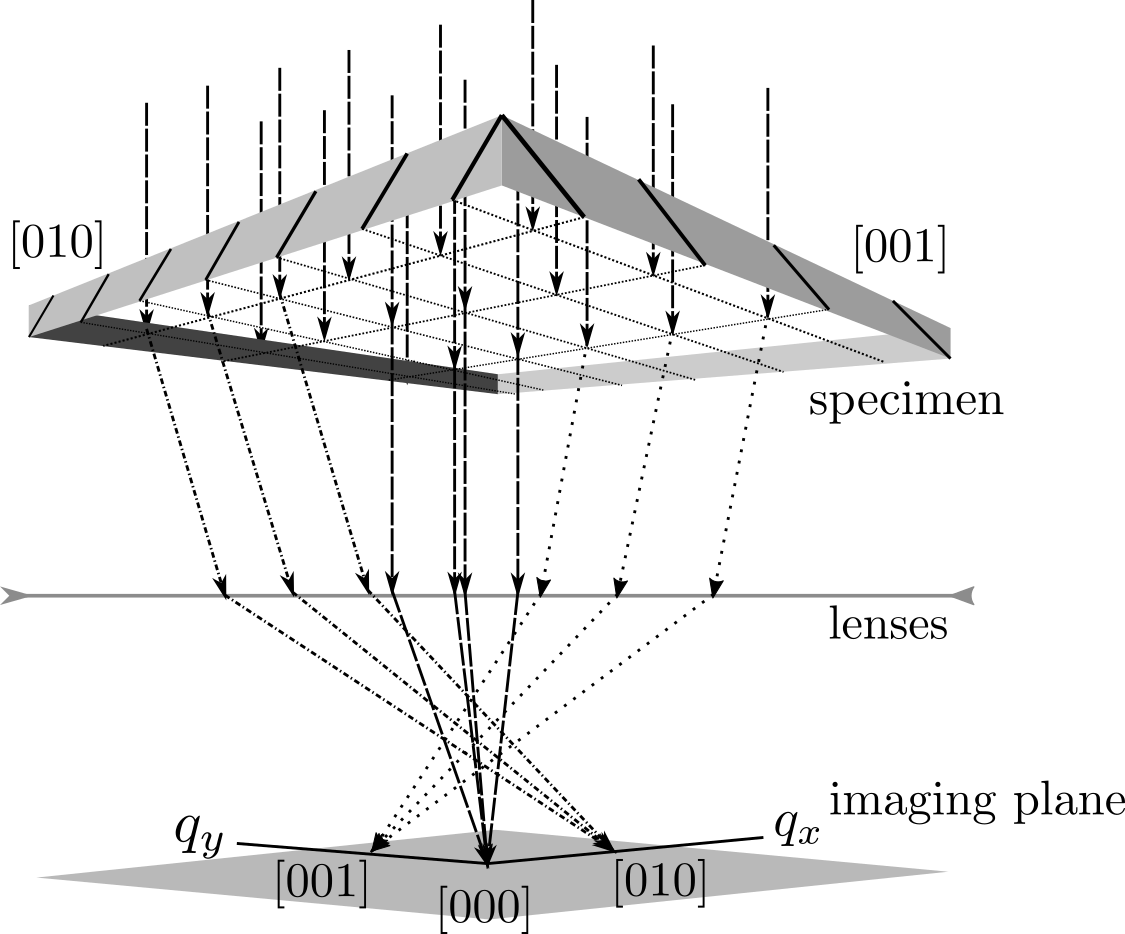
\includegraphics[width=0.75\linewidth, keepaspectratio]{diff-im3d.png}
	\caption{scat}
	\label{fig:diff-im3d}
\end{figure}
\subsubsection{Energy filtered transmission electron microscope}
\label{sec:eftem}
\subsection{Physical relevance of MREELS data}
\cite{doi:10.1021/acs.nanolett.9b03928}
\cite{doi:10.1021/acsphotonics.7b00103}
\cite{doi:10.1063/1.4921405}